\documentclass[compress,10pt,usenames,dvipsnames]{beamer}

\usecolortheme{beaver}
\useoutertheme{split}
\usefonttheme[onlymath]{serif}
\setbeamertemplate{headline}[default]
\setbeamertemplate{navigation symbols}{}
\mode<beamer>{\setbeamertemplate{blocks}[rounded][shadow=true]}
%\setbeamercovered{transparent}
\setbeamercolor{block body example}{fg=blue, bg=black!20}
\useoutertheme[subsection=false]{miniframes}

\usepackage[format=plain,textfont=it,up]{caption}
\usepackage{amsmath,amsthm,amsfonts,subcaption,graphicx,animate,hyperref,tikz,algorithm,algorithmic,tkz-euclide,animate,wasysym}
\usepackage{xcolor}
\usetikzlibrary{decorations.pathmorphing}

\captionsetup[algorithm]{labelformat=empty}

\theoremstyle{remark}
\newtheorem*{remark}{Remark}

\title{Surreal Trajectories and the Quantum Potential}
\author{David Darrow}
\institute{MIT}



\newcommand{\tens}[1]{\mathbf{\overset{\text{\scriptsize$\leftrightarrow$}}{#1}}}
\newcommand{\unit}[1]{\mathbf{\hat{#1}}}
\newcommand{\vc}[1]{\mathbf{#1}}
\newcommand{\ql}{\textquotedblleft}
\newcommand{\qr}{\textquotedblright{}}
\newcommand{\pdrv}[2]{\frac{\partial #1}{\partial #2}}
\newcommand{\tpdrv}[2]{\tfrac{\partial #1}{\partial #2}}
\newcommand{\drv}[2]{\frac{d #1}{d #2}}
\newcommand{\tdrv}[2]{\tfrac{d #1}{d #2}}
\newcommand{\eps}{\varepsilon}
\newcommand{\ol}[1]{{\overline{#1}}}
\newcommand{\id}[1]{{\indices{#1}}}
\newcommand{\sff}{\mathrm{I\hspace*{-1pt}I}}
\newcommand{\downto}{\searrow}
\newcommand{\upto}{\nearrow}

\begin{document}

\frame{\titlepage}

\begin{frame}\frametitle{Overview}
	
	\begin{block}{}
		\alert{Quantum Controversy! Background on Surreal Trajectories}
	\end{block}
	\only<2-3>{\begin{block}{}
		\alert{Surreal Walking Droplets \emph{in Silico}}
	\end{block}}
	\only<3>{\begin{block}{}
		\alert{Looking Ahead: the Hydrodynamic Quantum Potential}
	\end{block}}
\end{frame}

\section{Quantum Controversy!}
\begin{frame}\frametitle{ESSW Thought Experiment}
	\begin{figure}
		\centering
		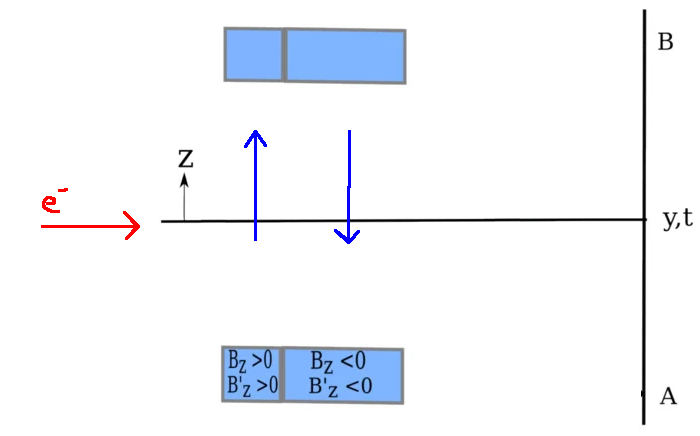
\includegraphics[scale=0.3]{Figures/diag0.png}
	\end{figure}
\end{frame}

\begin{frame}\frametitle{ESSW Thought Experiment}
	\begin{figure}
		\begin{subfigure}[t]{.6\textwidth}
			\vspace*{-1.5in}
			Integrating the system is straightforward:
			\begin{enumerate}
				\item<2-5> Reduce to 1D using classical approximation $y\sim t$.
				\item<3-5> Initialize as spin-right wavepacket.
				\item<4-5> Set $\hat{H} = (\hat{p}_z - q\hat{A}_z)^2 - q\hat{\sigma}_z\hat{B}_z$.
				\item<5> Solve by decomposing 
				\begin{align*}|\psi(z,t)\rangle &= \psi_+(z,t)\otimes|\!\uparrow\rangle \\
					&\quad+ \psi_-(z,t)\otimes|\!\downarrow\rangle.
				\end{align*}
			\end{enumerate}
		\end{subfigure}%
		\begin{subfigure}[t]{.4\textwidth}
			\centering
			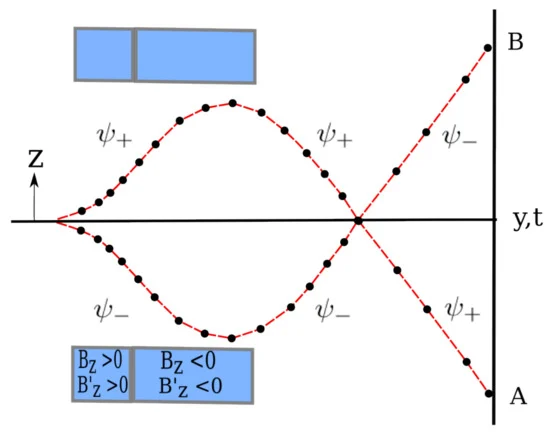
\includegraphics[scale=0.25]{Figures/diag1.png}
		\end{subfigure}
	\end{figure}
\end{frame}

\begin{frame}\frametitle{ESSW Thought Experiment}
	\begin{figure}
		\begin{subfigure}[t]{.6\textwidth}
			\vspace*{-1.5in}
			But, this contradicts the Bohmian picture!
			\begin{itemize}
				\item<2-3> Symmetry arguments show that the Bohmian velocity field is odd in $z$.
				\item<3> (ESSW, '92) calculated* the field directly, and found the right-hand picture.
			\end{itemize}
		\end{subfigure}%
		\begin{subfigure}[t]{.4\textwidth}
			\centering
			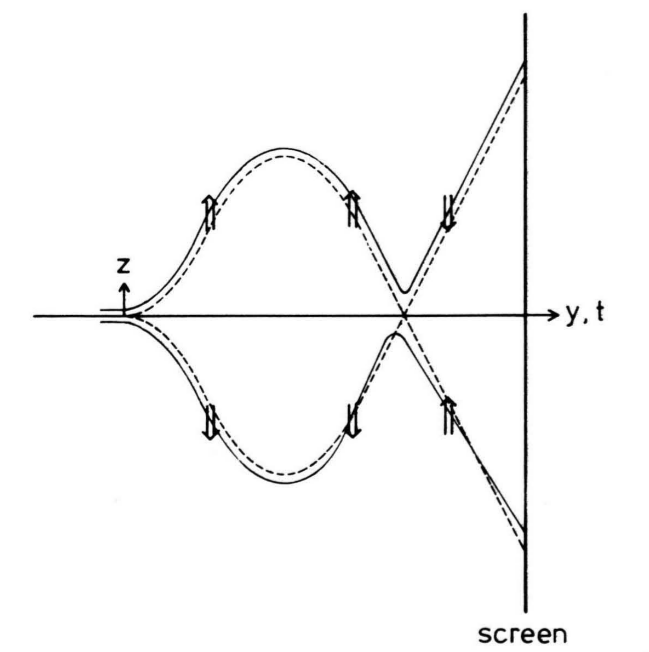
\includegraphics[scale=0.45]{Figures/fake_fig.png}
		\end{subfigure}
	\end{figure}
\end{frame}

\begin{frame}\frametitle{Possible Experimental Evidence?}
	\begin{figure}
		\begin{subfigure}[t]{.6\textwidth}
			\vspace*{-1.5in}
			\begin{itemize}
				\item[]<1-2> (ESSW, '92) suggests the shown experiment:\bigskip
				\item[]<2> They calculate that the \emph{top} sensor would be triggered, but the Bohmian trajectory goes along the \emph{bottom}.
			\end{itemize}
		\end{subfigure}%
		\begin{subfigure}[t]{.4\textwidth}
			\centering
			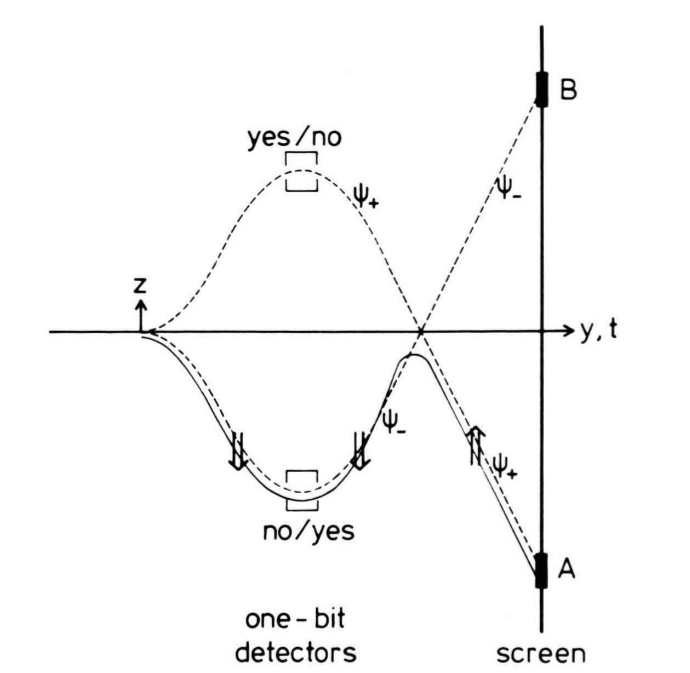
\includegraphics[scale=0.45]{Figures/fake_fig1.png}
		\end{subfigure}
	\end{figure}
\end{frame}

\begin{frame}
	This thought experiment shows that Bohmian mechanics is ``at variance with the actual: that is, the observed track'' (ESSW, '92).
	
	\bigskip
	\pause
	Moreover, it shows that Bohmian mechanics is ``at variance with common sense'' (Scully, '98).
\end{frame}


\begin{frame}\small
	There are a handful of issues with the analysis of ESSW:
	\begin{enumerate}\small
		\item<1-4> Their predicted wave packets are correct, but wave packet trajectories are distinct from particle trajectories.
		\item<2-4> They calculated trajectories using a spin-0 version of Bohmian mechanics.
		\item<3-4> They neglected to show probability currents in the Schrödinger picture (shown below, calculated in (Hiley and Reeth, '18)).
		\item<4> Bohmian mechanics is entirely equivalent to Schrödinger mechanics, and they cannot be mathematically or experimentally distinguished.
	\end{enumerate}

	\only<1-2>{
		
		\begin{figure}
			\phantom{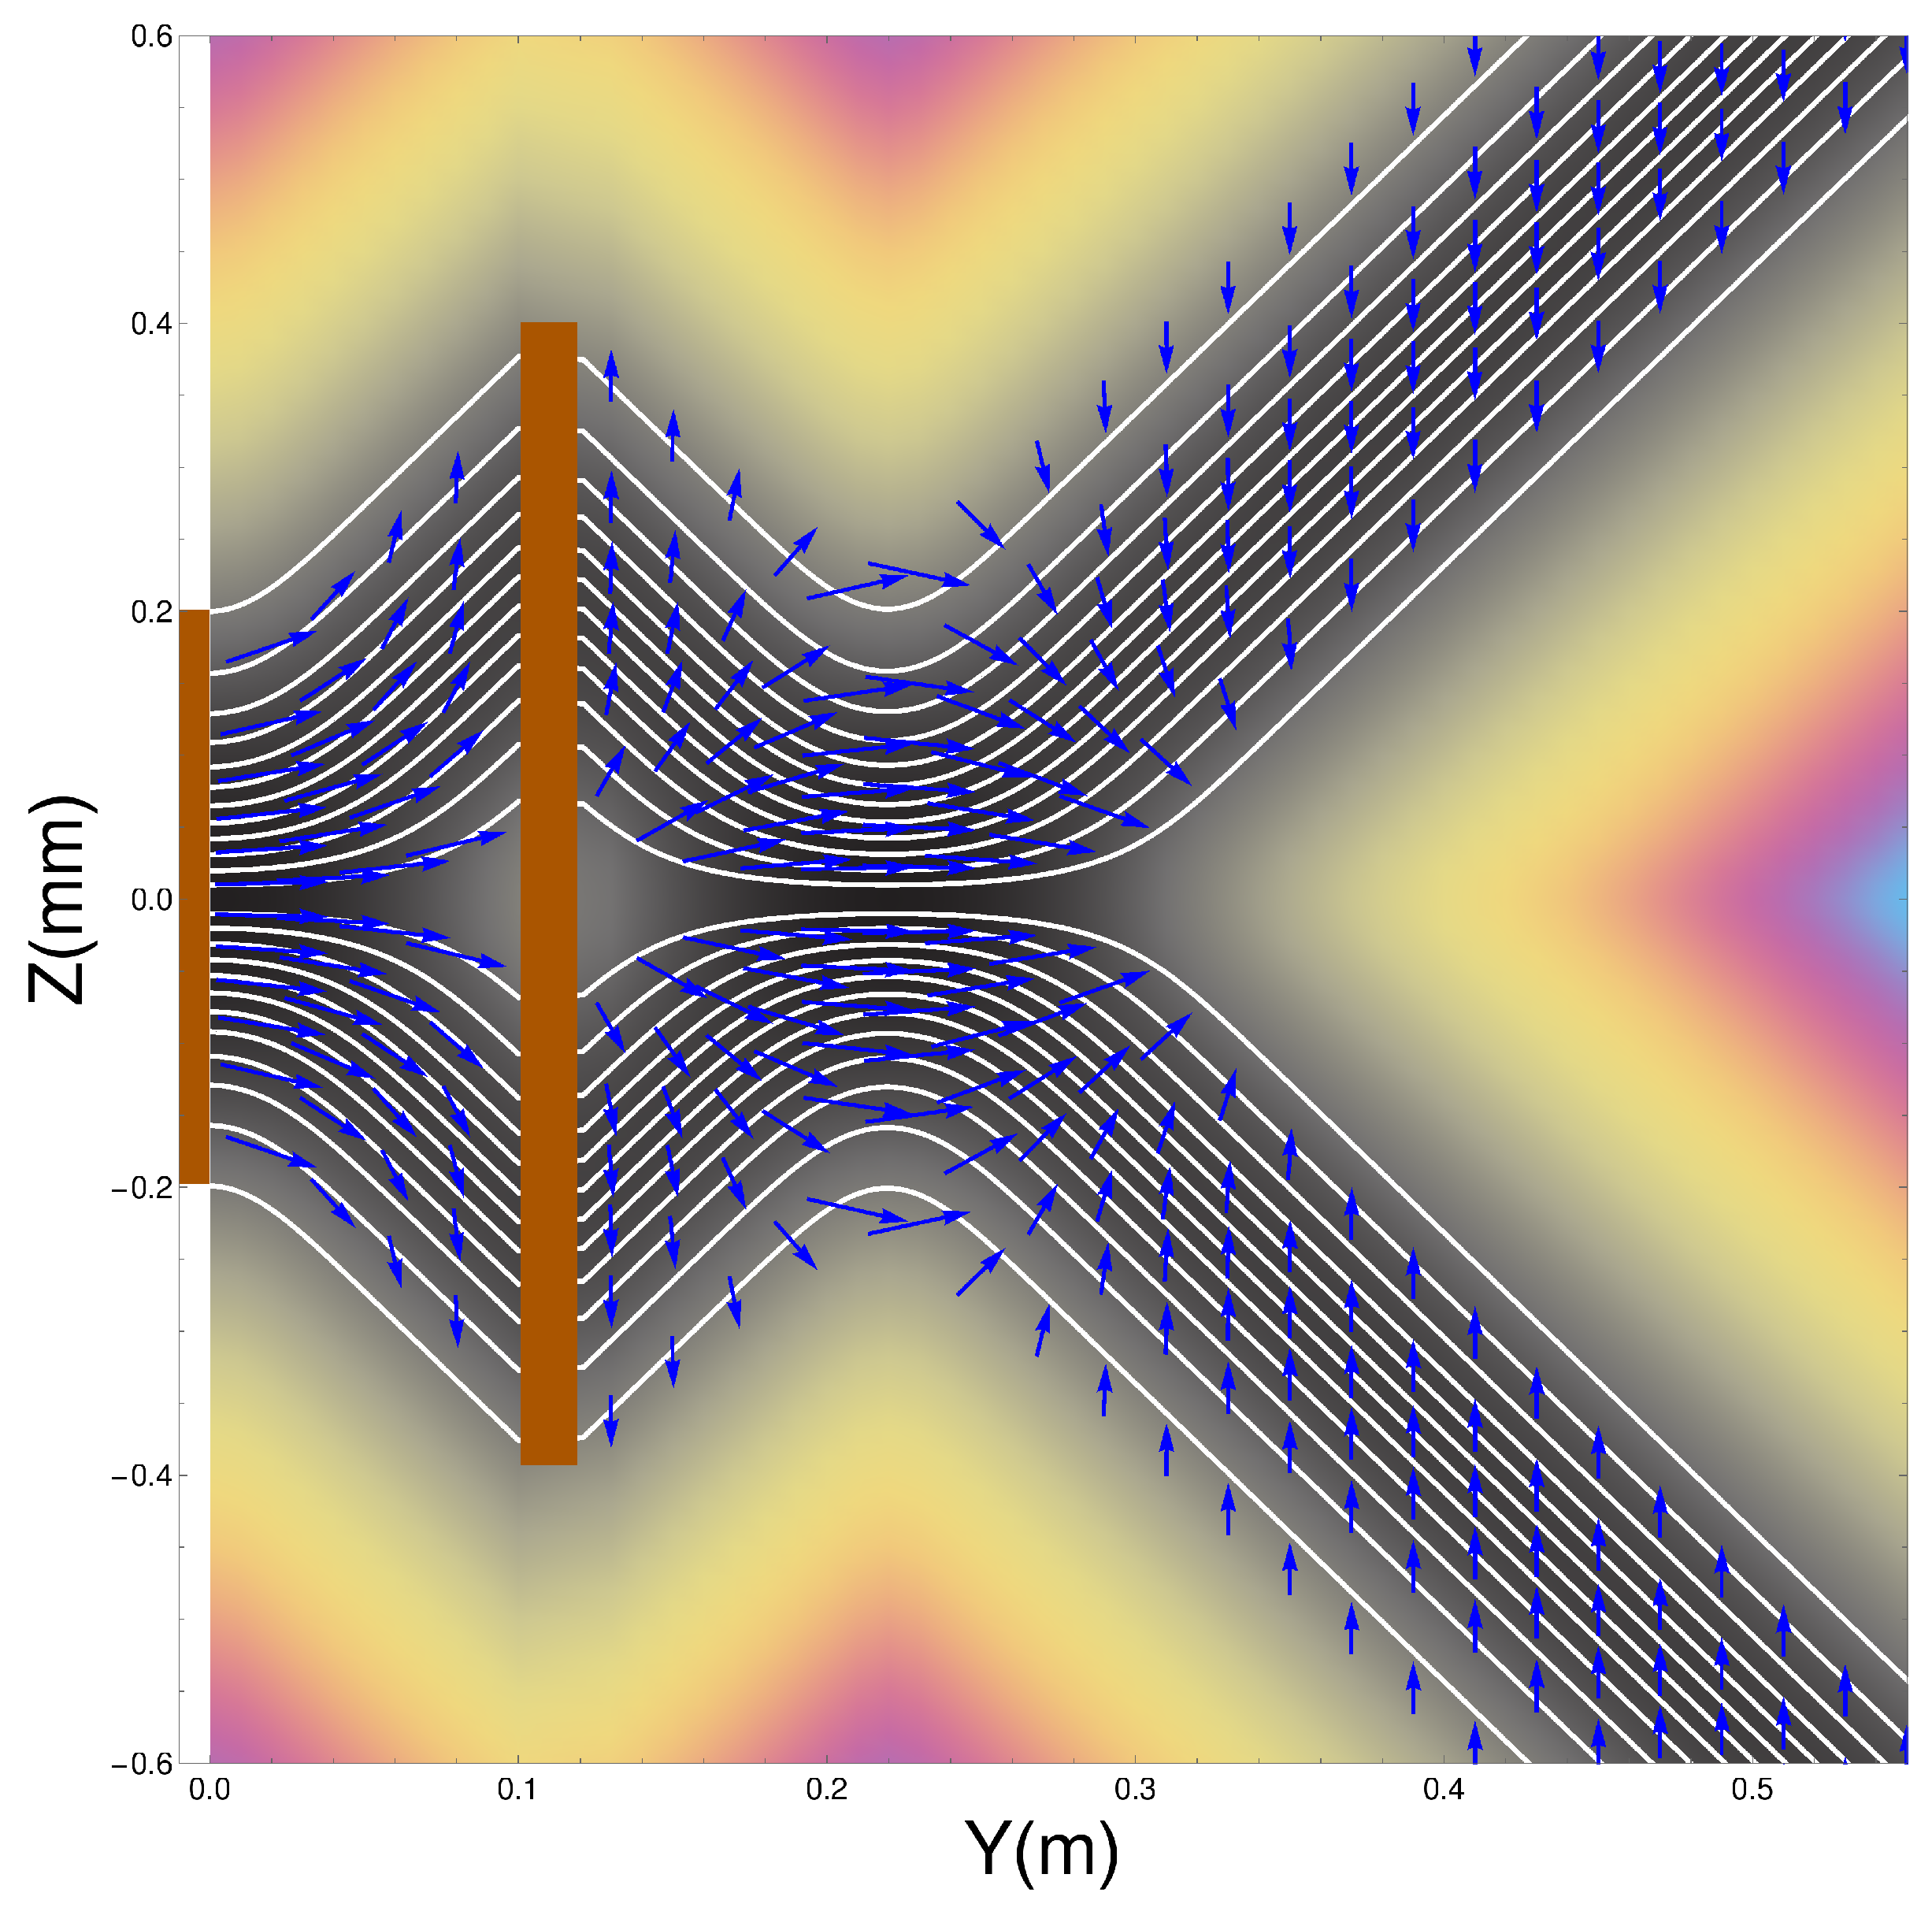
\includegraphics[scale=0.45]{Figures/good_fig.png}}
		\end{figure}
		
	}
	\only<3-4>{
	\begin{figure}
		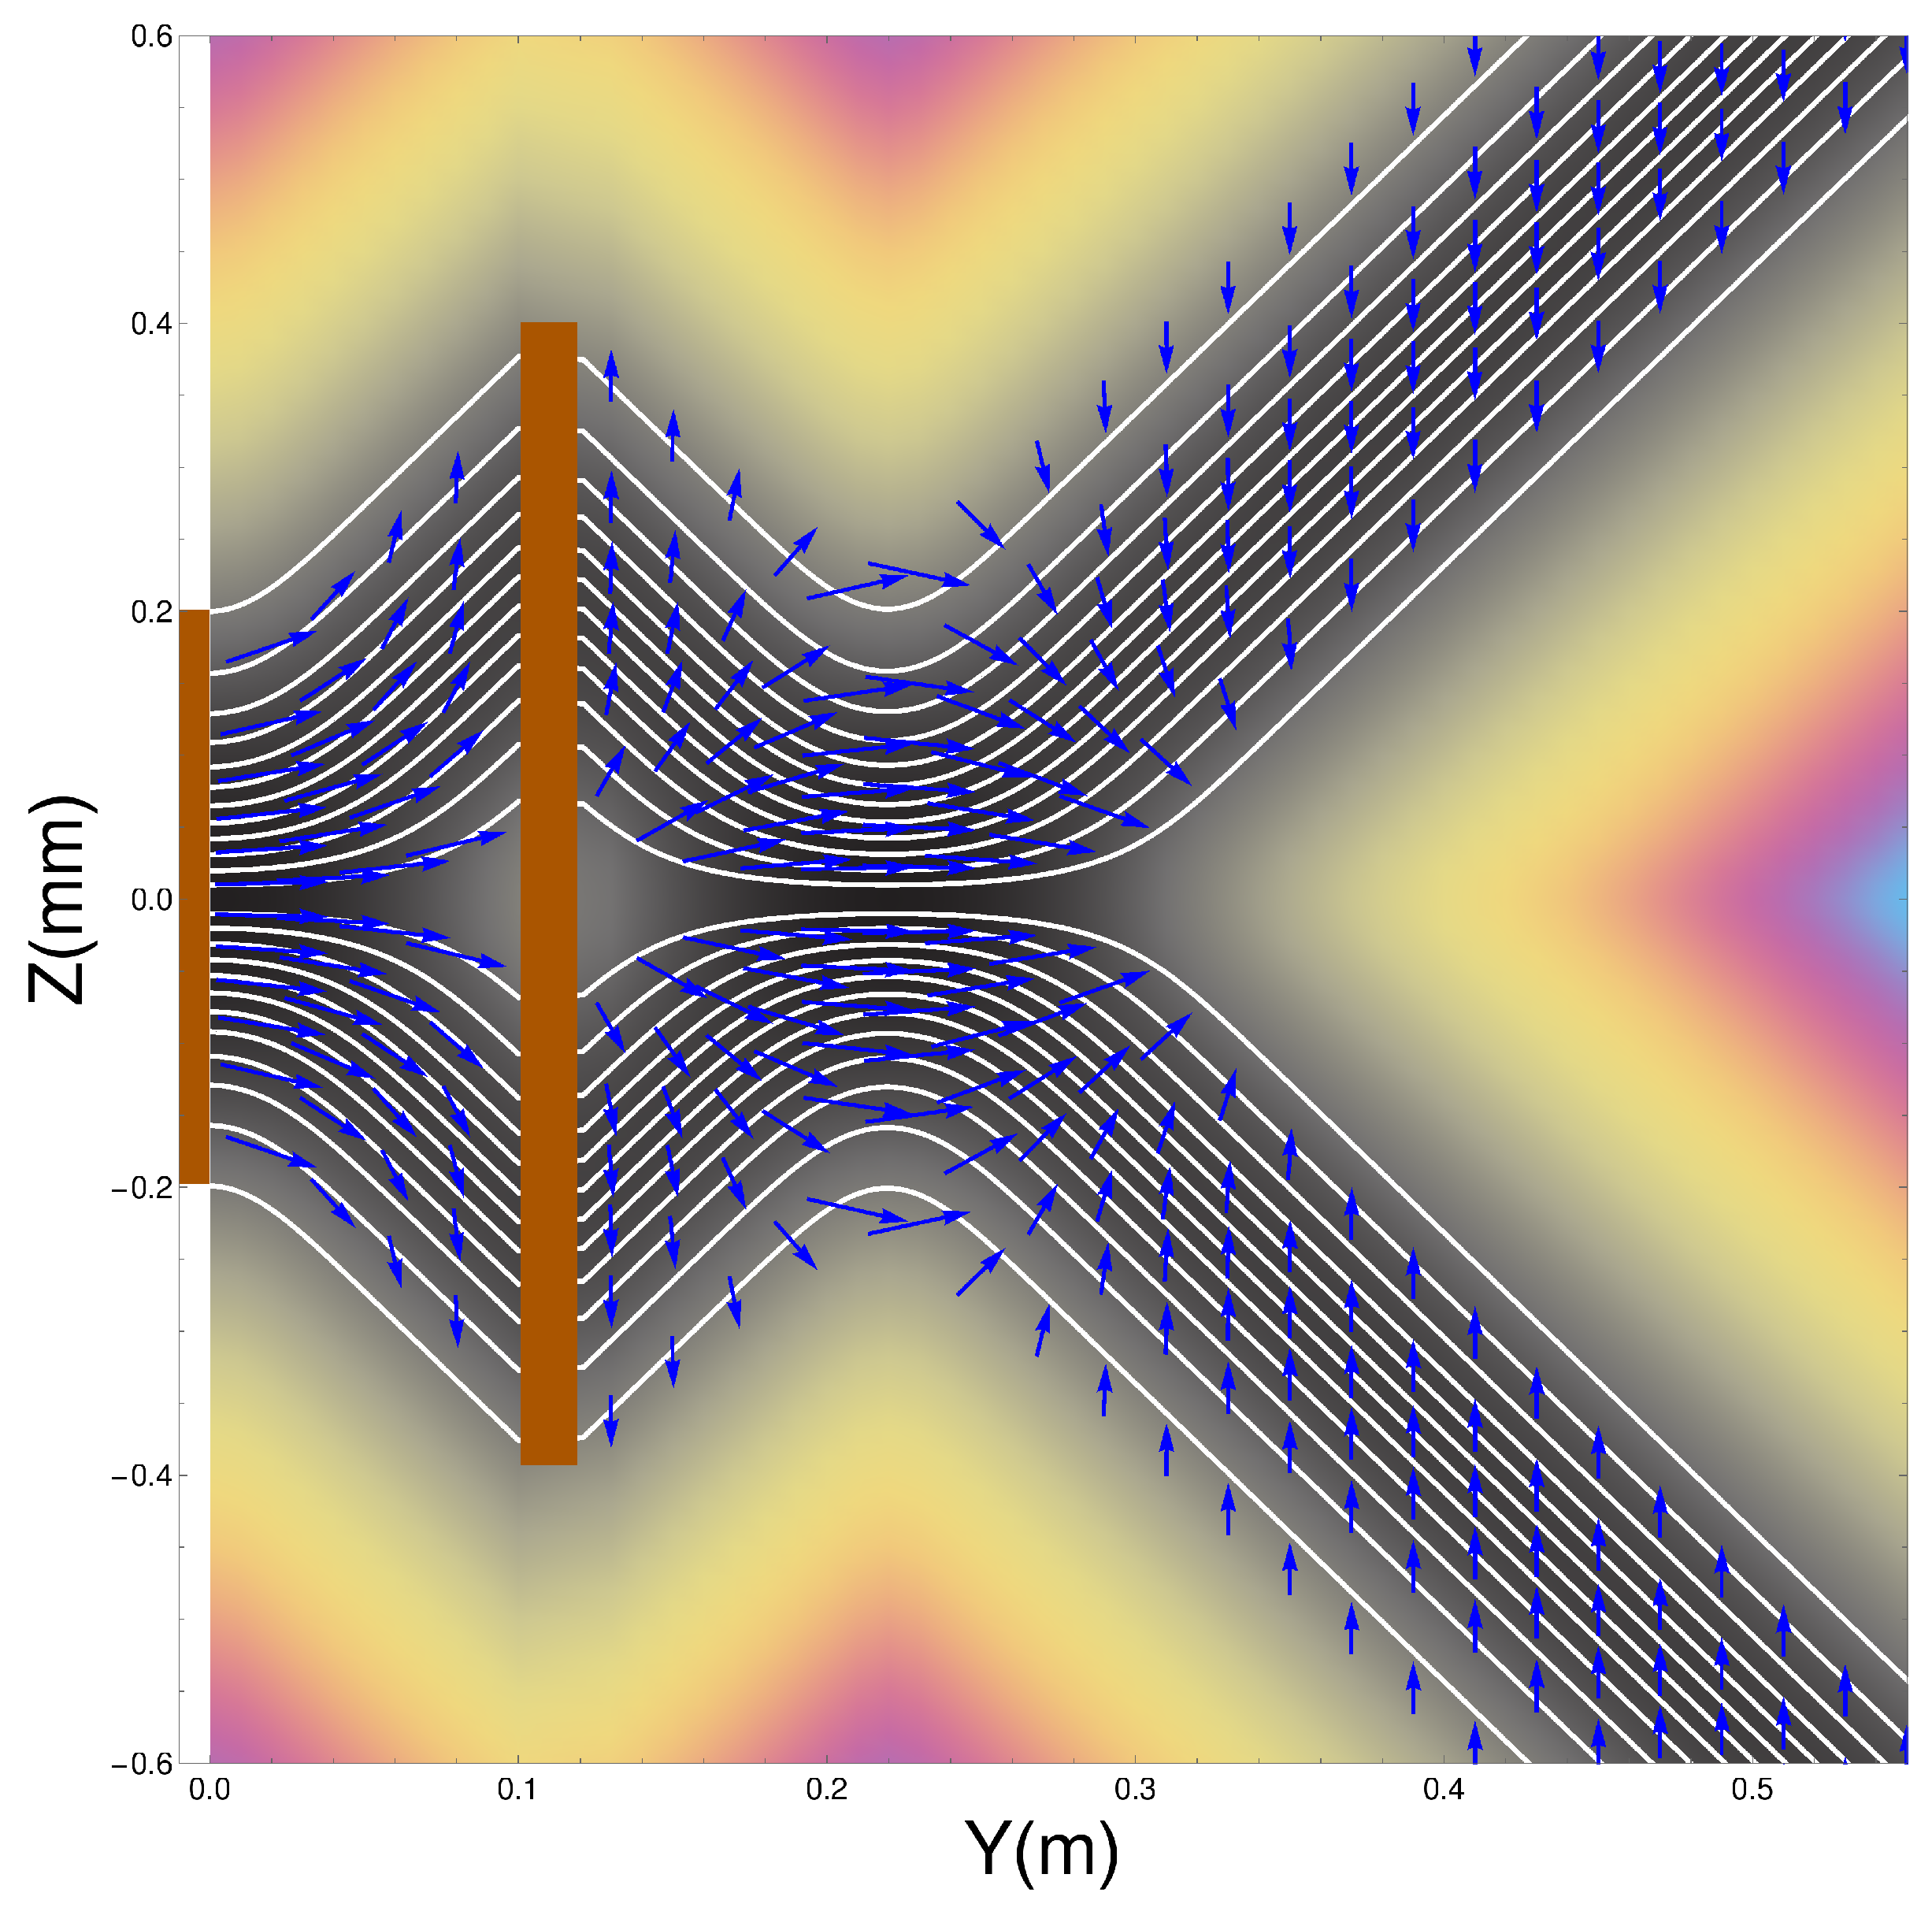
\includegraphics[scale=0.45]{Figures/good_fig.png}
	\end{figure}
	}
\end{frame}

\begin{frame}\frametitle{Takeaways}
	\begin{itemize}
		\item <2-4> Surreal trajectories are \emph{not} a problem in quantum mechanics.
		\item <3-4> Surreal trajectories are not unique to Bohmian mechanics.
		\item <4> Nothing is unique to Bohmian mechanics.
	\end{itemize}
\end{frame}

\section{Numerical Simulations}
\begin{frame}\frametitle{Can we replicate this?}
	To try to replicate these dynamics \emph{in silico}, we used a modified version of the code from (Faria, 2017).
	
	\begin{figure}
		\begin{subfigure}[t]{.5\textwidth}
			\centering
			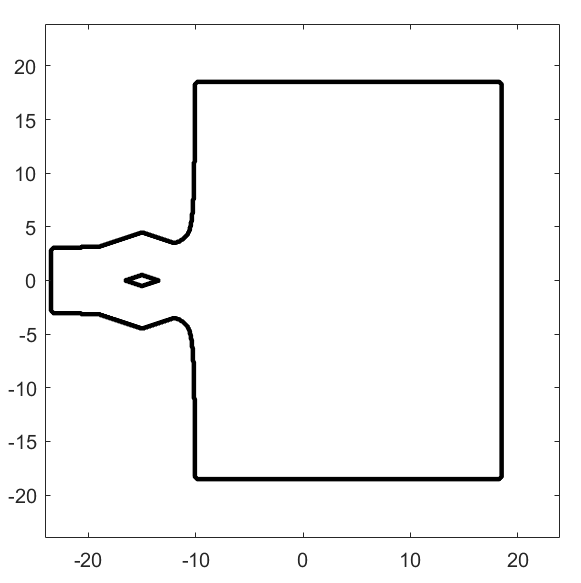
\includegraphics[scale=0.25]{Figures/setup.png}
			
		\end{subfigure}%
		\begin{subfigure}[t]{.5\textwidth}
			\vspace*{-1.5in}
			\begin{itemize}
				\item $T_F = \lambda_F = 1$
				\item $\text{memory} = 0.905$
				\item $r_\text{drop} = 3.9\times 10^{-4}$
				\item $w_\text{channel} = 6$
				\item $\ell_\text{channel} = 13$
			\end{itemize}
		\end{subfigure}
	\end{figure}
\end{frame}

\begin{frame}\frametitle{Can we replicate this?}
	To try to replicate these dynamics \emph{in silico}, we used a modified version of the code from (Faria, 2017).
	
	\begin{figure}
		\begin{subfigure}[t]{.5\textwidth}
			\centering
			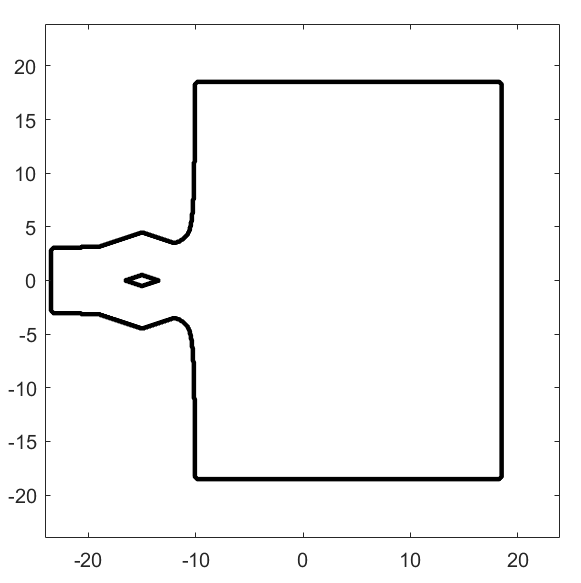
\includegraphics[scale=0.25]{Figures/setup.png}
			
		\end{subfigure}%
		\begin{subfigure}[t]{.5\textwidth}
			\vspace*{-1.5in}
			\begin{itemize}
				\item $T_F = \lambda_F = 1$
				\item $\text{memory} = 0.905$
				\item $r_\text{drop} = 3.9\times 10^{-4}$
				\item $w_\text{channel} = 6$
				\item $\ell_\text{channel} = 13$
			\end{itemize}
		\end{subfigure}
	\end{figure}
\end{frame}

\begin{frame}\frametitle{Yes, we can replicate this}
	\begin{figure}
		\begin{subfigure}[t]{.5\textwidth}
			\centering
			\includegraphics[scale=0.35]{Figures/fig1_nowall.png}
			
		\end{subfigure}%
		\begin{subfigure}[t]{.5\textwidth}
			\centering
			\includegraphics[scale=0.35]{Figures/fig1_yeswall.png}
		\end{subfigure}
	\end{figure}
\end{frame}

\begin{frame}\frametitle{Dependence on Memory}
	\begin{figure}
		\begin{subfigure}[t]{.33\textwidth}
			\centering
			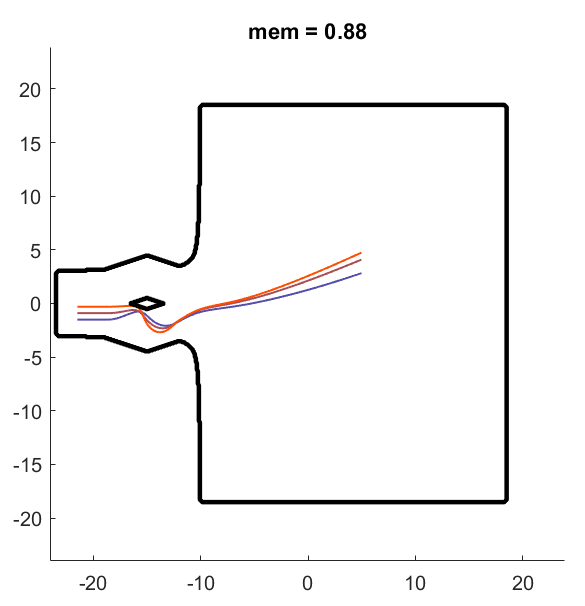
\includegraphics[scale=0.25]{Figures/mem1.png}
			
		\end{subfigure}%
		\begin{subfigure}[t]{.33\textwidth}
			\centering
			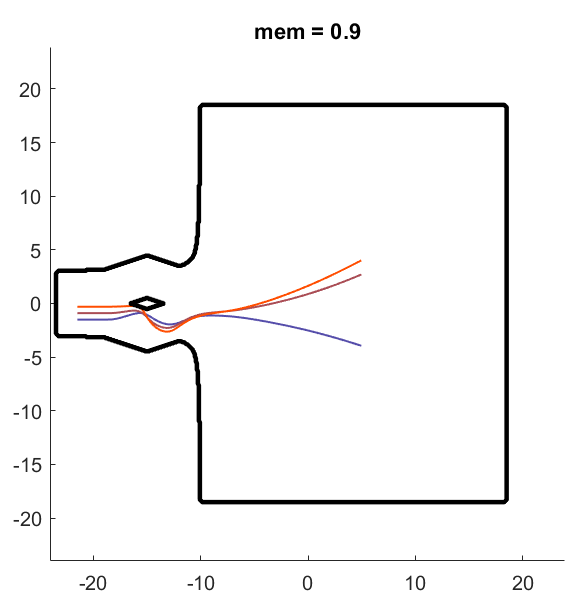
\includegraphics[scale=0.25]{Figures/mem2.png}
			
		\end{subfigure}%
		\begin{subfigure}[t]{.33\textwidth}
			\centering
			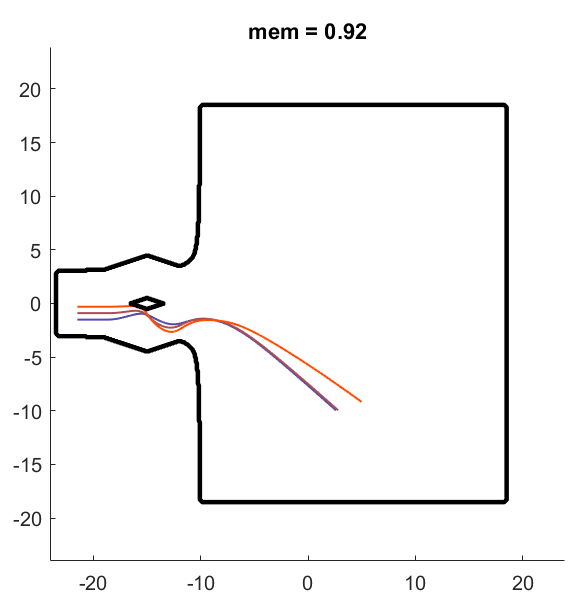
\includegraphics[scale=0.25]{Figures/mem3.png}
		\end{subfigure}
	\end{figure}
\bigskip
Note (not displayed): at high memory, we see surreal trajectories without the bottom reflector, because of the finite domain.
\end{frame}

\begin{frame}\frametitle{Dependence on Impact Parameter}
	\begin{figure}
		\centering
		\includegraphics[scale=0.4]{Figures/array.png}
	\end{figure}
\end{frame}

\section{Hydrodynamic Quantum Potential}

\begin{frame}\frametitle{The Quantum Potential}
	How do we connect the walking droplet to the quantum picture?
	\bigskip
	\pause
	
	The Bohmian picture evolves according to a set of Hamilton--Jacobi equations:
	\[\dot{\rho} + \nabla\cdot(\rho\nabla S) = 0,\]
	\[\dot{S} + \|\nabla S\|^2 = -V - \rho^{-1/2}\nabla\rho^{1/2}.\]
	\smallskip
	\pause
	
	This is simply a statistical Newtonian system with velocity field $\mathbf{J}=\nabla S$ and an extra, nonlocal potential
	\[V_\text{q} = \rho^{-1/2}\nabla\rho^{1/2}.\]
\end{frame}

\begin{frame}\frametitle{$V_q$ Examples:}
	\begin{figure}
		\begin{subfigure}[t]{.5\textwidth}
			\centering
			$ $
		\end{subfigure}%
		\begin{subfigure}[t]{.5\textwidth}
			\centering
			\only<1>{\phantom{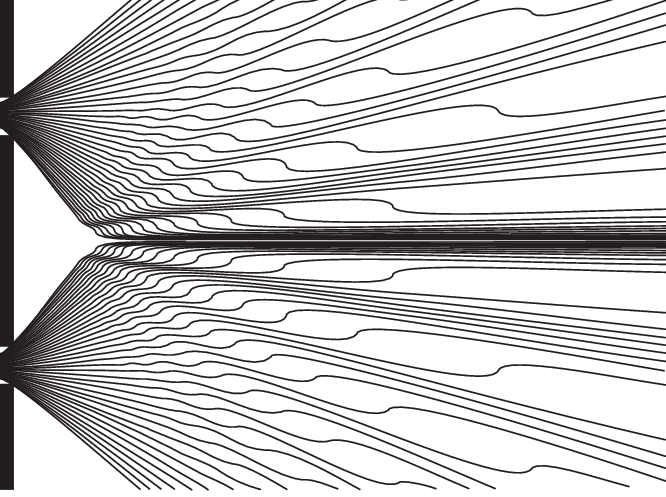
\includegraphics[scale=0.15]{Figures/potential_slits.png}}}
			\only<2-3>{
			\caption*{(Philippidis et al., '79)}
			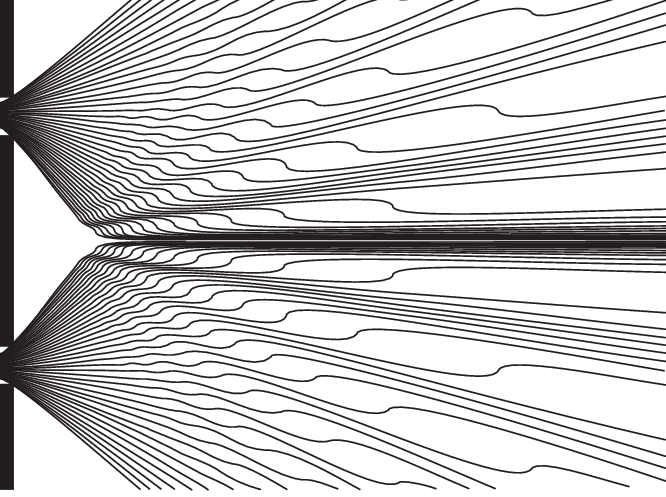
\includegraphics[scale=0.15]{Figures/potential_slits.png}
			}
		\end{subfigure}
		\begin{subfigure}[t]{.5\textwidth}
			\centering
			\vspace*{-2.25in}
			\caption*{(Hiley and Reeth, '18)}
			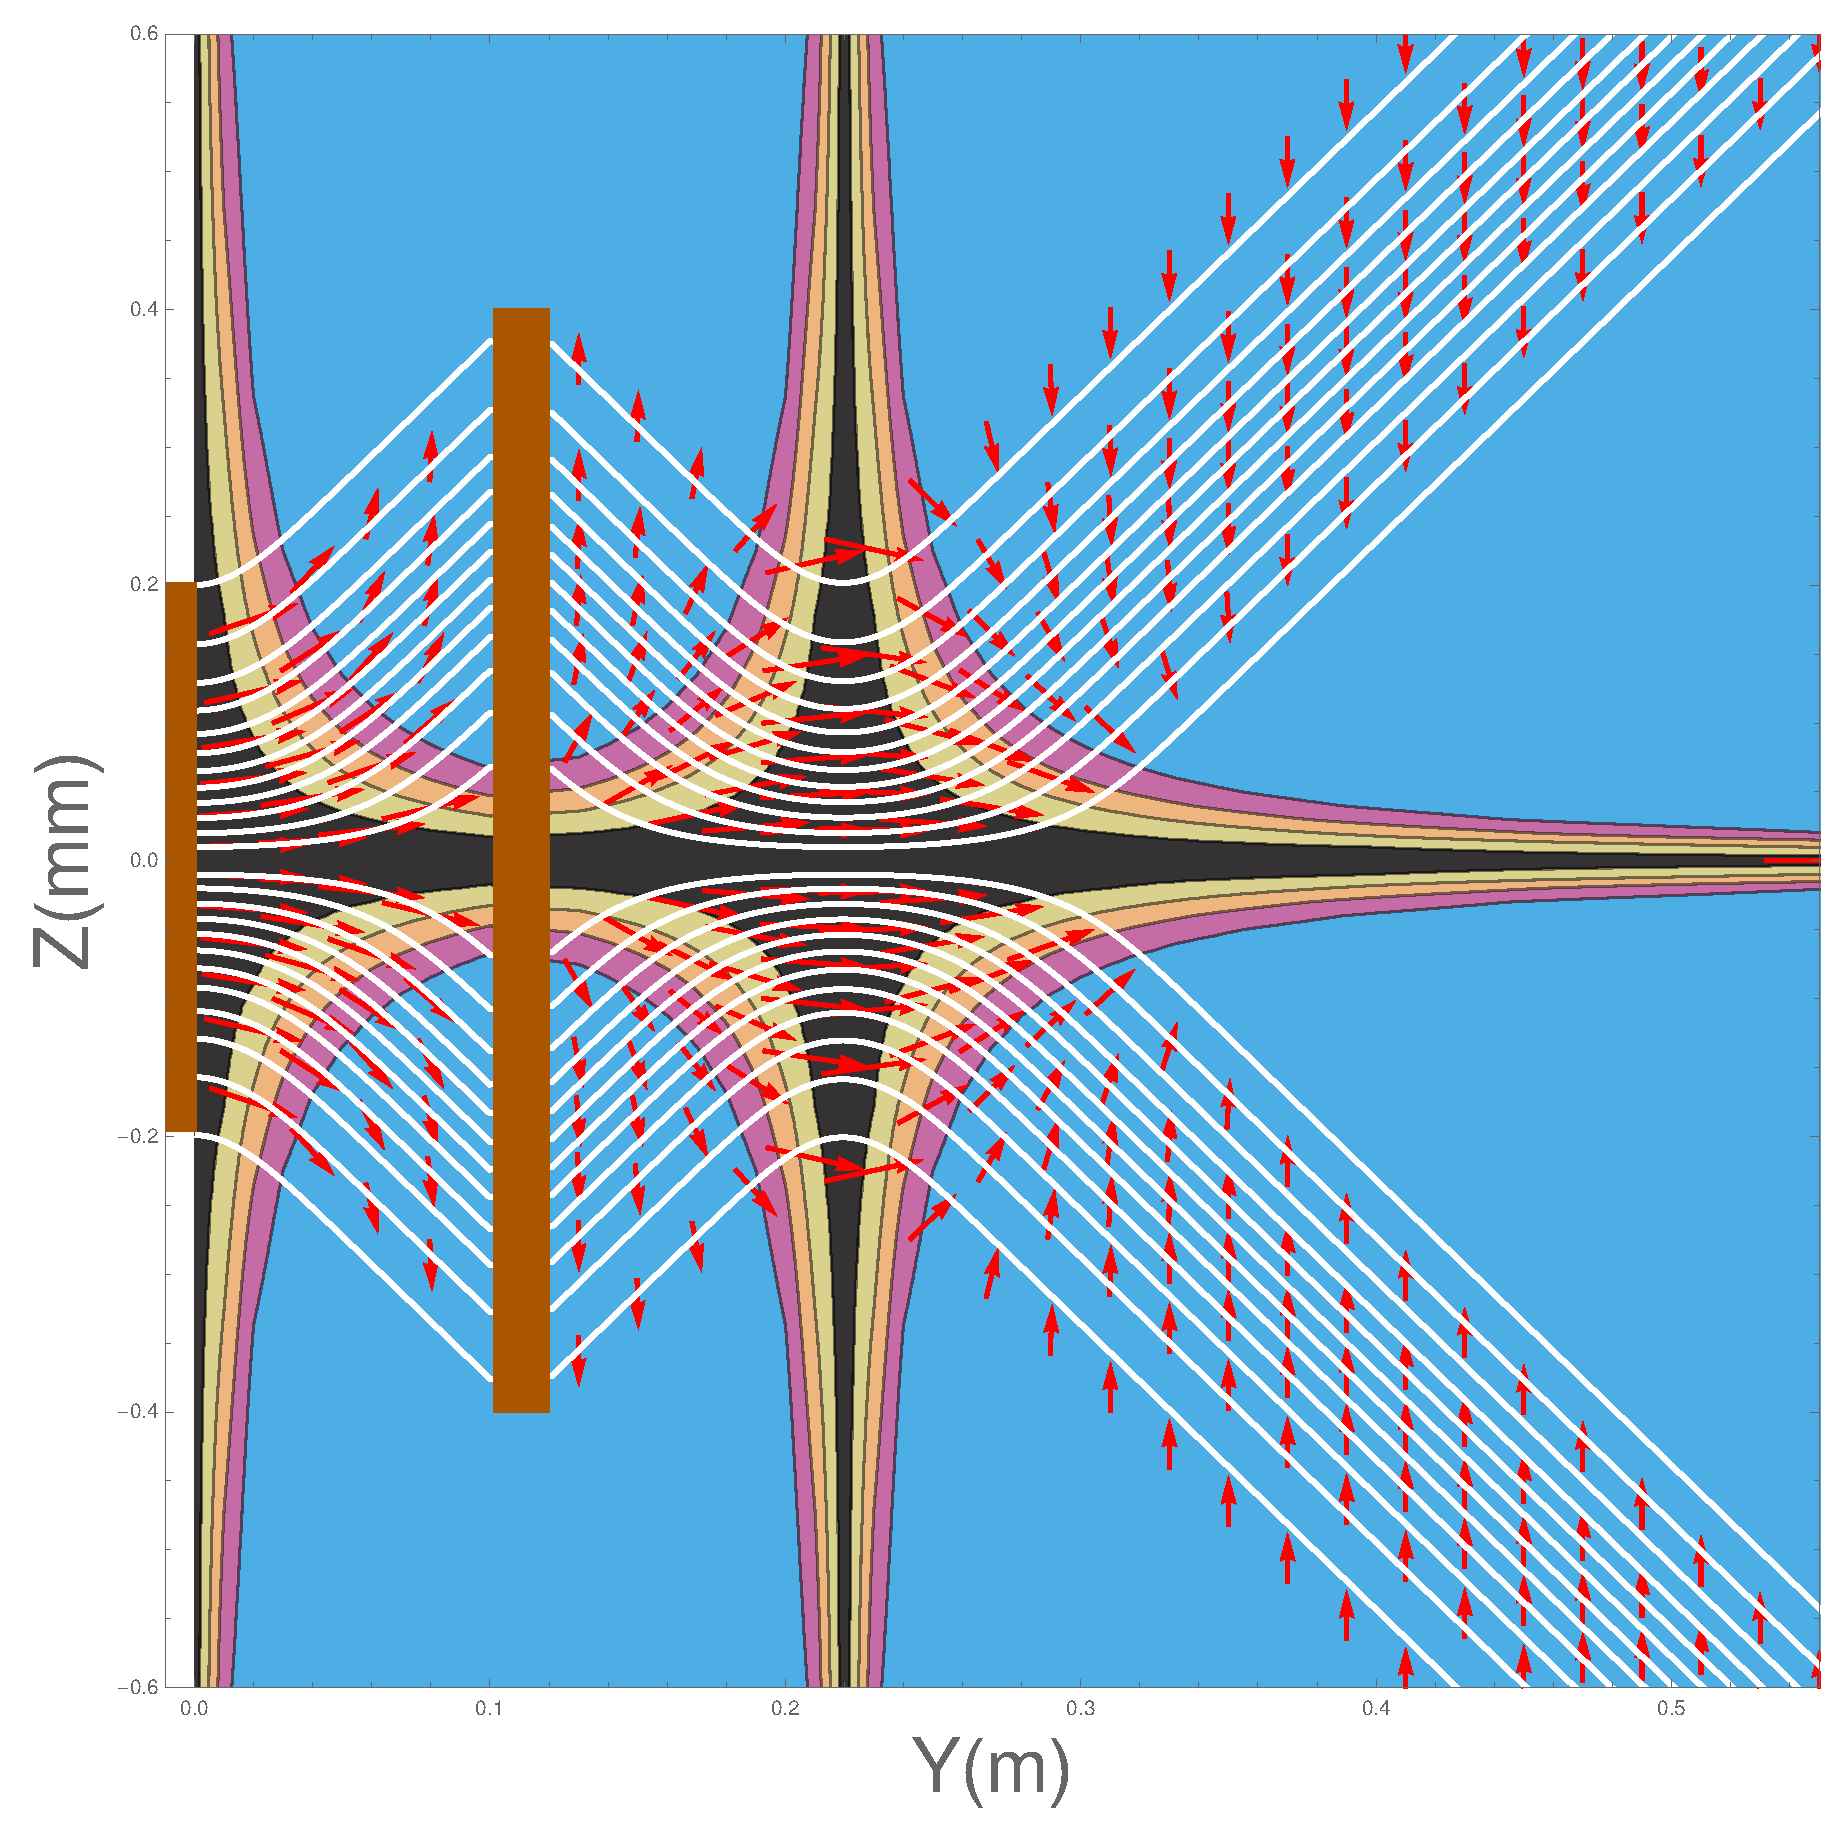
\includegraphics[scale=0.08]{Figures/potential_surreal.png}
			
		\end{subfigure}%
		\begin{subfigure}[t]{.25\textwidth}
			\centering
			\only<1>{\phantom{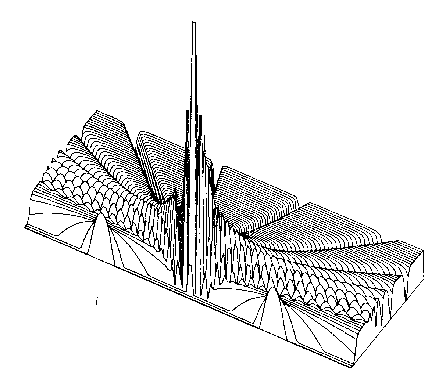
\includegraphics[scale=0.15]{Figures/potential_slits1.png}}}
			\only<2-3>{
			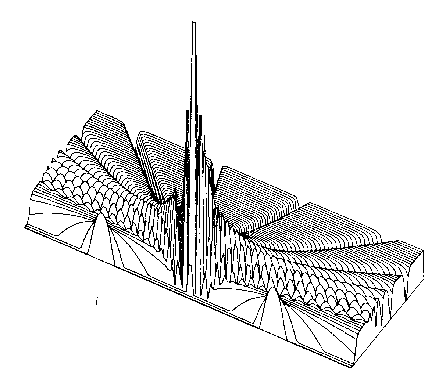
\includegraphics[scale=0.15]{Figures/potential_slits1.png}
		}
		\end{subfigure}%
		\begin{subfigure}[t]{.25\textwidth}
			\centering
			\only<1>{\phantom{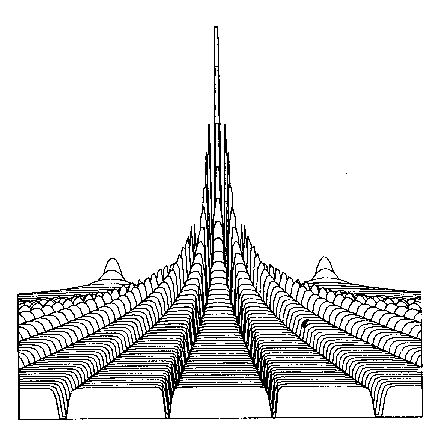
\includegraphics[scale=0.15]{Figures/potential_slits2.png}}}
			\only<2-3>{
			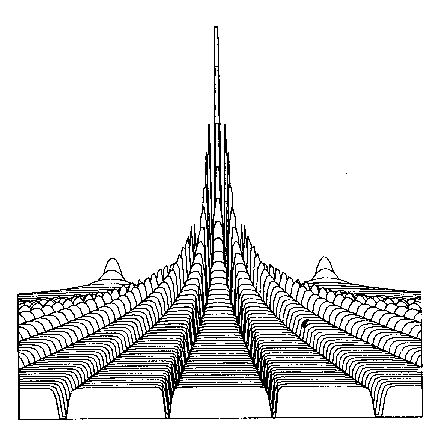
\includegraphics[scale=0.15]{Figures/potential_slits2.png}
		}
		\end{subfigure}
	\end{figure}
	\pause\pause
	It is important to note that these are all \emph{1-dimensional} quantum potentials, with a $y\sim t$ axis cutting across them.
\end{frame}

\begin{frame}\frametitle{$V_q\sim\langle \text{wave height}\rangle$}
	\begin{figure}
		\begin{subfigure}[t]{.5\textwidth}
			\centering
			\includegraphics[scale=0.3]{Figures/potential1.png}
			
		\end{subfigure}%
		\begin{subfigure}[t]{.5\textwidth}
			\centering
			\includegraphics[scale=0.3]{Figures/potential.png}
		\end{subfigure}
	\end{figure}
	\pause
	Note similar features:
	\begin{itemize}
		\item Vertical beams following the reflectors
		\item Horizontal beam to the right
		\item Large peaks at points of reconvergence
		\item ``Diffraction-like'' front at the right
	\end{itemize}
\end{frame}

\begin{frame}\frametitle{Other Possibilities?}
	Of course, the similarities here are rudimentary. What could be more fitting?
	\begin{itemize}
		\item<2-5> 1-D replica of walking droplet
		\item<3-5> Mapping out particle trajectories themselves
		\item<4-5> Heatmaps of stored momentum in field
		\item<5> Splices---rather than averages---of wave heights
	\end{itemize}
\end{frame}

\end{document}
